\section{Model Sequence and Geometry-Anchored Texture Learning}\label{sec:models}
\subsection{TREAD-ONE and Motivating Diagnostics}
TREAD-ONE is a custom 1,372,159-parameter network trained from scratch at an input resolution of $512\times384$ (height by width). A texture encoder, two context transformer blocks, and shared decoding features support two sigmoid masks, mask-derived boxes, six ordered boundary coordinates, and proxy classification. Twelve nonnegative latent maps are combined with a detached, normalized predicted-tread gate and signed linear class weights. Their additive contributions plus bias reconstruct the class logits. This identity makes score accounting inspectable; it does not establish semantic concepts or input-level causal faithfulness.\AIdraftingnote

The three selected seeds achieved strong internal mask agreement but inconsistent proxy transfer. We therefore evaluated a matched seed-1 shared-gradient intervention. Classification is one task and the weighted dense objective the second. When shared gradients have a negative dot product, each is projected away from the other using the original pair of vectors; the projected gradients are then combined. This is a declared symmetric two-task variant motivated by gradient surgery \cite{pcgrad}. It preserves task routing, but global gradient clipping can still affect the total update. Its results do not support promotion over the matched baseline.

ATLAS then freezes the dense anchor and uses local query/reference evidence for proxy classification. The first version showed appearance sensitivity and repeated exposure to a restricted query set. ATLAS-LC introduces paired local-contrast grayscale inputs, full-source-hash self-exclusion from an 18-image reference bank, and square-root component sampling. ATLAS-CONTEXT adds a zero-initialized, bounded positional residual over a frozen LC prior. These changes address distinct observed weaknesses, yet none recovers low-category recall on the historical test role. They are context for the texture question, not interchangeable causal ablations of one factor.

GEO, the geometry-first revision, separates geometry, texture, and annotation-error parameters. Its bounded geometry adjustment preserves mask quality and modestly improves internal point error. Its texture representation remains ineligible under the joint gate. A 64-dimensional diversity projector is also difficult to interpret with centered batches of eight, whose covariance rank cannot exceed seven. This dimensional constraint is a feasibility observation, not proof that it caused the failed representation. TRACE retains GEO's fixed final geometry and reduces the auxiliary projector to six dimensions while replacing learned texture targets with explicit fixed descriptors.

\subsection{Canonical Atlas and Fixed Targets}\label{sec:targets}
TRACE uses 1,399,227 frozen geometry parameters and 71,022 trainable texture parameters, for 1,470,249 total. The geometry consists of the selected TREAD-ONE anchor and GEO's final geometry adjustment. GEO's final state was not selected under its original joint gate; its use here is an explicitly frozen research dependency, not a retrospective promotion.

Predicted tyre--tread support defines a canonical $512\times256$ atlas, sampled with bilinear red--green--blue (RGB) values and nearest-neighbor support. Source rows narrower than 16 pixels are unavailable. The atlas contains an $8\times4$ grid of nonoverlapping $64\times64$ tiles. All dimensions in this paper use height before width.

Within each tile, grayscale $g=(R+G+B)/3$ is locally standardized using masked $9\times9$ means and standard deviations, with denominator floor 0.02. The result is clipped to $[-3,3]$, divided by three, and multiplied by observation support to obtain $z$. Tile-local Sobel derivatives $d_x,d_y$, divided by eight, supply edge information. Table~\ref{tab:targets} defines the six fields. These fixed descriptors encode canonical image structure; their thresholds and coordinates have no calibrated physical-wear interpretation.

\begin{table}[t]
\caption{Six fixed image fields before cell averaging. $e=d_x^2+d_y^2$; $\Delta$ is the four-neighbor Laplacian.}\label{tab:targets}
\centering\small
\begin{tabularx}{\columnwidth}{lL}\toprule
Field & Definition\\\midrule
Contrast & $z$\\
Gradient energy & $\sqrt{e}$\\
Orientation axis & $(d_x^2-d_y^2)/(e+0.0025)$\\
Orientation cross & $2d_xd_y/(e+0.0025)$\\
Relative curvature & $\min\{1,|\Delta z/4|/(|d_x|+|d_y|+0.05)\}$\\
Contrast occupancy & $\mathbf{1}[|z|>0.15]$\\\bottomrule
\end{tabularx}
\end{table}

Loss support intersects predicted support with the complement of the annotation ignore mask. An $11\times11$ erosion with invalid padding removes pixels whose radius-five contrast/derivative dependency is not valid. Each tile is reduced to $4\times4$ cells of $16\times16$ pixels. A cell is available only when at least 64 valid pixels remain; the count weights its loss. Missing targets have zero weight and are not treated as observed zeros.

Channel means and population standard deviations are fitted on the 386 training images using 64-bit floating-point (FP64) accumulation and stored in 32-bit floating point (FP32), with a standard-deviation floor of 0.001. Targets are standardized with these statistics. A separate train-position mean is retained for each tile/cell/channel, including its count and availability. Neither statistic uses validation or historical-test targets.

\subsection{Local, Contextual, and Global Paths}\label{sec:architecture}
Figure~\ref{fig:architecture} separates the paths that are easily conflated in aggregate metrics. Input channels are $z,d_x,d_y$, and gradient magnitude. Four stride-two convolution blocks, with channel widths 16, 24, 32, and 48, Group Normalization, and sigmoid linear unit (SiLU) activations, produce a 48-dimensional vector per tile after spatial averaging. Let $Z\in\mathbb{R}^{32\times48}$ denote these local tokens. A shared multilayer decoder
\begin{equation}
 D:\mathbb{R}^{48}\rightarrow\mathbb{R}^{96}\rightarrow\mathbb{R}^{96}
\end{equation}
uses SiLU between its two linear layers and reshapes each output to six $4\times4$ fields. The local prediction is $D(Z)$, before cross-tile mixing or global pooling.

\begin{figure*}[t]
\centering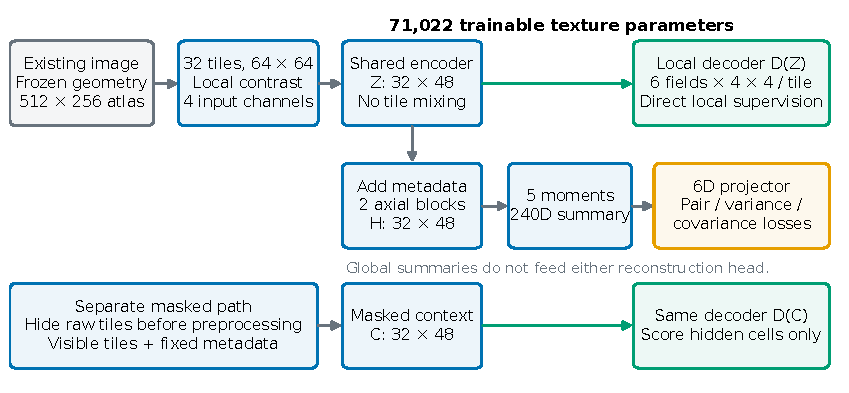
\includegraphics[width=\textwidth]{architecture.pdf}
\caption{Actual TRACE information flow. The local reconstruction head reads unpooled tokens $Z$. The masked head reads contextual tokens $C$ from a separately masked observation path. The full-context tokens $H$ feed an auxiliary global summary. Thus local reconstruction can be useful while the global summary fails diversity requirements. Geometry remains frozen in all paths.}\label{fig:architecture}
\end{figure*}

Row, column, and predicted coverage metadata are projected into 48 dimensions. Two residual axial blocks mix depthwise row and column convolutions with pointwise channel transformations, producing full-context tokens $H$. Coverage is normalized within each supported band and then equally across supported bands to yield nonnegative masses $m_t$ with $\sum_t m_t=1$. The recorded local mean is $\sum_t m_t Z_t$; the full-context mean is $\sum_t m_t H_t$.

The actual global descriptor contains five moments of $H$. Coordinates $y$ and $x$ are the fixed linearly spaced values from $-1$ to $1$ on the eight rows and four columns. With
\begin{equation}
 b_t=[1,y_t,x_t,y_tx_t,y_t^2-1/3],
\end{equation}
the descriptor concatenates $\sum_t m_t b_{tk}H_t$ for $k=1,\ldots,5$, yielding 240 dimensions. The constant $1/3$ is source-defined; the discrete basis is not assumed orthogonal under each image's masses. A $240\rightarrow48\rightarrow6$ projector supplies the paired-view diversity objective. It does not feed the local decoder.

\subsection{Masking, Objective, and Original Selection}\label{sec:training}
Two deterministic image/view-addressed photometric views vary brightness, contrast, and gamma in $[0.9,1.1]$, while targets remain those of the clean atlas. A separate plan hides one supported tile in a band when at least two exist, for at most eight hidden tiles. Hidden raw RGB and observation support are removed \emph{before} preprocessing and encoding. A learned mask token and the permitted position/coverage metadata then enter the context blocks, producing $C$. The masked prediction $D(C)$ is scored on hidden supported cells. Clean targets, annotation ignore masks, and full-path encodings are not context inputs. However, the fixed predicted geometry was computed from the full image; the masking boundary is conditional on that geometry and is not a claim of image-level causal occlusion.

The loss is
\begin{equation}\label{eq:loss}
\begin{split}
\mathcal{L}={}&\mathcal{L}_{\mathrm{local}}+\mathcal{L}_{\mathrm{mask}}
 +0.1\mathcal{L}_{\mathrm{pair}}\\
 &+0.1\mathcal{L}_{\mathrm{var}}+0.01\mathcal{L}_{\mathrm{cov}}.
\end{split}
\end{equation}
Reconstruction uses Smooth L1 with transition $\beta=0.1$ on standardized fields. Valid-pixel counts weight cells; channels are averaged within each image and available images are then averaged equally. The two views' terms are averaged. The pair term is mean squared error between six-dimensional projected vectors. With unbiased sample covariance $S$ ($n-1$ denominator), the variance term averages $\max(0,0.1-\sqrt{S_{jj}+10^{-4}})$, and the covariance term is $\sum_{j\ne k}S_{jk}^2/(6\cdot5)$. Diversity losses require at least seven eligible rows, making six-dimensional centered variation feasible in batches of eight. This is an adaptation inspired by VICReg, not a claim to reproduce its original recipe.

TRACE uses AdamW with learning rate 0.001, weight decay 0.0001, gradient clipping at one, FP32 arithmetic, and no scheduler or gradient scaler. One seed is run for 60 epochs and 49 updates per epoch. Each epoch has 386 primary image draws and six deterministic padding draws, yielding 23,520 draws in total. Kaggle provides two T4 graphics processing units (GPUs): geometry-cache construction uses the second device and texture optimization the first. This is not distributed data-parallel training.

Three controls predict hidden descriptors: the training channel mean, the training position mean, and the mean of visible descriptors in the same band. All are scored on the same intersection of supported hidden cells and control availability. The original validation contract requires at least 90\% primary exposure and 95\% common control coverage; at least 5\% masked improvement over \emph{each} control; at least 10\% local improvement over the position control; projector rank at least four and median standard deviation at least 0.05; local-mean and spatial-summary ranks at least four; and within-component local/spatial ranks at least two. Finite-state and frozen-geometry provenance checks also apply. Eligible checkpoints minimize masked loss divided by the strongest control loss, plus 0.1 times paired cosine distance, retaining the earliest tie. No epoch is eligible, so the selected endpoint remains unavailable. The final epoch is studied as a fixed diagnostic endpoint.
